\documentclass{beamer}

\usepackage[utf8]{inputenc}
\usepackage[english]{babel}
\usepackage{graphicx}
\usepackage{color}
\usepackage{natbib}
\usepackage{amssymb}
\usepackage{algorithm}
\usepackage{algpseudocode}
\usepackage{caption}

\usepackage{amsmath}
\usepackage{tikz}
\usetikzlibrary{arrows,calc,tikzmark,shapes.misc}

\tikzset{every picture/.style=remember picture}
% Define a TikZ node for math content:
\newcommand{\mathnode}[2]{%
  \mathord{\tikz[baseline=(#1.base), inner sep = 0pt]{\node (#1) {$#2$};}}}

\DeclareMathOperator*{\argmin}{arg\,min}
\DeclareMathOperator*{\argmax}{arg\,max}


% Beamer layout
\hypersetup{colorlinks=True, citecolor=green, linkcolor=blue}

\let\oldbibitem=\bibitem
\renewcommand{\bibitem}[2][]{\label{#2}\oldbibitem[#1]{#2}}
\let\oldcite=\cite
\renewcommand\cite[1]{\hyperlink{#1}{\oldcite{#1}}}
\let\oldcitep=\citep
\renewcommand\citep[1]{\hyperlink{#1}{\oldcitep{#1}}}
\let\oldciteauthor=\citeauthor
\renewcommand\citeauthor[1]{\hyperlink{#1}{\oldciteauthor{#1}}}

\usetheme{boxes}
\beamertemplatenavigationsymbolsempty
\setbeamertemplate{sections/subsections in toc}[circle]
\setbeamertemplate{footline}[frame number]
\setbeamertemplate{itemize items}[circle]
\setbeamertemplate{itemize subitem}[square]

% Front slide
\title{{\bf Approximating likelihood ratios with calibrated classifiers}}
\author{
Gilles Louppe\\
{\it ATLAS ML workshop}
}
\date{March 31, 2016}

\begin{document}

\begin{frame}[plain]
\titlepage
\end{frame}

\begin{frame}
    \centering
    Joint work with
    \vspace{2em}

    \begin{columns}
      \begin{column}[t]{0.45\textwidth}
        \centering
        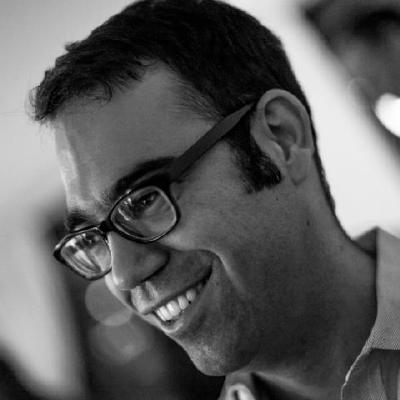
\includegraphics[height=10em]{figures/kyle.jpg}\\
        Kyle Cranmer\\
        {\scriptsize New York University}
      \end{column}
      \begin{column}[t]{0.45\textwidth}
          \centering
          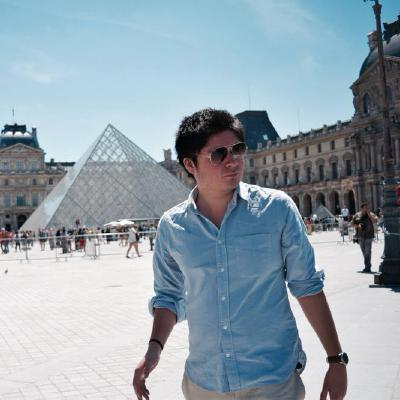
\includegraphics[height=10em]{figures/juan.jpg}\\
          Juan Pavez\\
          {\scriptsize Federico Santa Mar\'ia University}
      \end{column}
    \end{columns}

    \vspace{2em}

    See \citep{cranmer2015approximating} for full details.
\end{frame}

\begin{frame}
    \frametitle{Likelihood-free setup}

    \begin{itemize}
        \item Complex simulator $p$ parameterized by $\theta$;
        \item Samples $\mathbf{x} \sim p$ can be generated on-demand;
        \item ... but the likelihood $p(\mathbf{x}|\theta)$ cannot be evaluated!
    \end{itemize}

    \centering
    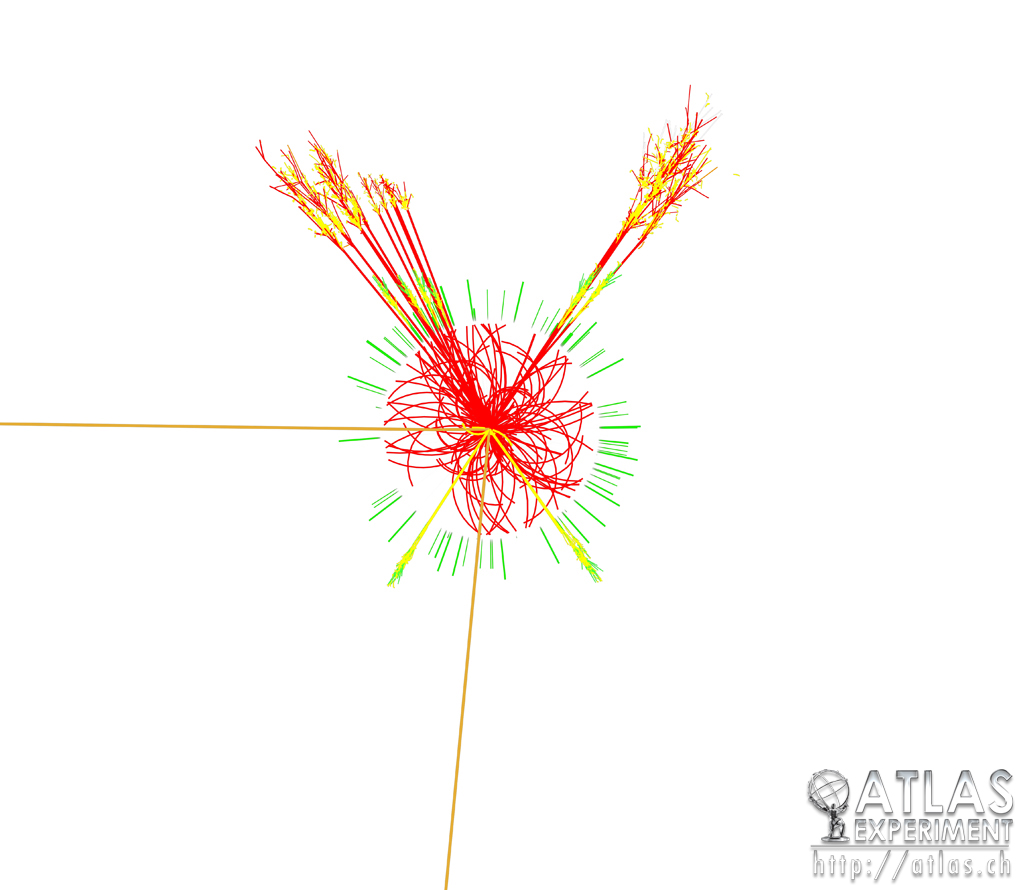
\includegraphics[height=10em]{figures/sim-boson.jpg}

\end{frame}

\begin{frame}
    \frametitle{Simple hypothesis testing}

    \begin{itemize}
        \item Assume some observed data ${\cal D} = \{ \mathbf{x}_1, \dots, \mathbf{x}_n \}$;
        \item Test a null $\theta = \theta_0$ against an alternative $\theta = \theta_1$;
        \item The Neyman-Pearson lemma states that the most powerful test statistic is
            $$
            \lambda({\cal D}; \theta_0, \theta_1) = \prod_{\mathbf{x} \in {\cal D}} \frac{ p_\mathbf{X}(\mathbf{x}|\theta_0)}{ p_\mathbf{X}(\mathbf{x}|\theta_1)}.
            $$
        \item ... but neither $p_\mathbf{X}(\mathbf{x}|\theta_0)$ nor $p_\mathbf{X}(\mathbf{x}|\theta_1)$ can be evaluated!

    \end{itemize}

\end{frame}

\begin{frame}[fragile]
    \frametitle{Straight approximation}

    \begin{enumerate}
        \item Approximate $p_\mathbf{X}(\mathbf{x}|\theta_0)$ and $p_\mathbf{X}(\mathbf{x}|\theta_1)$ individually, using density estimation algorithms;
        \item Evaluate their ratio $r(\mathbf{x};\theta_0,\theta_1)$.
    \end{enumerate}

    \vspace{1em}

    Because of the curse of dimensionality, this is a too difficult problem!

    $$
      \mathnode{A}{  \frac{ p_\mathbf{X}(\mathbf{x}|\theta_0)}{ p_\mathbf{X}(\mathbf{x}|\theta_1)} } = \mathnode{B}{ r(\mathbf{x};\theta_0,\theta_1)}
    $$

    \begin{tikzpicture}[overlay]
      \path [>=stealth, ->, shorten <= 3pt, shorten >=3 pt, blue]
        (A) edge [bend left=60] (B);
      \path [>=stealth, ->, shorten <= 3pt, shorten >=3 pt, red]
        (B) edge [bend left=60] node {$/$} (A);
    \end{tikzpicture}

    \vspace{1em}

    {\centering \it When solving a problem of interest, do not solve a more general problem as an intermediate step. -- Vladimir Vapnik}

\end{frame}

\begin{frame}
    \frametitle{Approximating likelihood ratios with classifiers}

    \begin{itemize}
        \item The likelihood ratio is invariant under the change of variable $\mathbf{U} = s(\mathbf{X})$, provided $s(\mathbf{x})$ is monotonic with $r(\mathbf{x})$.

        $$
        r(\mathbf{x};\theta_0,\theta_1) = \frac{ p_\mathbf{X}(\mathbf{x}|\theta_0)}{ p_\mathbf{X}(\mathbf{x}|\theta_1)} = \frac{ p_\mathbf{U}(s(\mathbf{x})|\theta_0)}{ p_\mathbf{U}(s(\mathbf{x})|\theta_1)}
        $$

        \item Well, a classifier trained to distinguish $\mathbf{x} \sim p_0$ from $\mathbf{x} \sim p_1$ yields a decision function $s(\mathbf{x})$ which is monotonic with $r(\mathbf{x})$.

        \item Estimating $p(s(\mathbf{x})|\theta)$ is now easy, since the change of variable $s(\mathbf{x})$ projects $\mathbf{x}$ in a 1D space, where only the informative content of the ratio is preserved.

        \item Disentangle training from calibration.
    \end{itemize}
\end{frame}

\begin{frame}
    \frametitle{Inference and composite hypothesis testing}

    Approximated likelihood ratios can be used for inference, as

    {\small
    \begin{align}\label{eqn:mle}
        \hat{\theta} &= \argmax_\theta  p({\cal D} | \theta) \nonumber \\
                     &= \argmax_\theta  \prod_{\mathbf{x} \in {\cal D}} \frac{p(\mathbf{x}| \theta)}{p(\mathbf{x}|\theta_1)} \nonumber \\
                     &= \argmax_\theta  \prod_{\mathbf{x} \in {\cal D}} \frac{p(s(\mathbf{x}; \theta, \theta_1) | \theta)}{p(s(\mathbf{x}; \theta, \theta_1) |\theta_1)} \;
    \end{align}}

    where $\theta_1$ is fixed and $s(\mathbf{x}; \theta, \theta_1)$ is a family of classifiers parameterized by $(\theta, \theta_1)$.

    \vspace{1em}

    Accordingly, generalized (or profile) likelihood ratio tests can be evaluated in the same way.
\end{frame}

\begin{frame}
    \frametitle{Parameterized learning}

    For inference, we need to build a family $s(\mathbf{x}; \theta, \theta_1)$ of classifiers.

    \begin{itemize}
        \item One could build a classifier $s$ independently for all $\theta, \theta_1$. But this is computationally expensive and would not guarantee a smooth evolution of $s(\mathbf{x}; \theta, \theta_1)$ as $\theta$ varies.

        \item Solution: build a single parameterized classifier instead, where parameters are defined as additional input features.
    \end{itemize}

    {\scriptsize
    \begin{algorithmic}
        \State ${\cal T := \{ \}}$;
        \While{ $\text{size}({\cal T}) < N $ }
            %\State Select or draw $\theta_0$, $\theta_1$ from $\Theta_0$, $\Theta_1$;
            \State Draw $\theta_0 \sim \pi_{\Theta_0}$;
    	    \State Draw $\mathbf{x} \sim p(\mathbf{x}|\theta_0)$;
    		\State ${\cal T} := {\cal T} \cup \{ ((\mathbf{x}, \theta_0, \theta_1), y=0) \}$;
            \State Draw $\theta_1 \sim \pi_{\Theta_1}$;
    		\State Draw $\mathbf{x} \sim p(\mathbf{x}|\theta_1)$;
    		\State ${\cal T} := {\cal T} \cup \{ ((\mathbf{x}, \theta_0, \theta_1), y=1) \}$;
        \EndWhile
        \State Learn a single classifier $s(\mathbf{x}; \theta_0, \theta_1)$ from ${\cal T}$.
    \end{algorithmic}}

\end{frame}

\begin{frame}
    \frametitle{Example: Inference from multidimensional data}

\begin{columns}
    \begin{column}{0.55\textwidth}
       Let assume 5D data $\mathbf{x}$ generated
       from the following process $p_0$:

            {\scriptsize
           \begin{enumerate}
               \item $\mathbf{z} := (z_0, z_1, z_2, z_3, z_4)$, such that
                   $z_0 \sim {\cal N}(\mu=\alpha, \sigma=1)$,
                   $z_1 \sim {\cal N}(\mu=\beta, \sigma=3)$,
                   $z_2 \sim {\text{Mixture}}(\frac{1}{2}\,{\cal N}(\mu=-2, \sigma=1), \frac{1}{2}\,{\cal N}(\mu=2, \sigma=0.5))$,
                   $z_3 \sim {\text{Exponential}(\lambda=3)}$, and
                   $z_4 \sim {\text{Exponential}(\lambda=0.5)}$;
               \item $\mathbf{x} := R  \mathbf{z}$, where $R$ is a fixed
               semi-positive definite $5 \times 5$ matrix defining a fixed projection
               of $\mathbf{z}$ into the observed space.
           \end{enumerate}}

        Our goal is to infer the values $\alpha$ and $\beta$ based on ${\cal D}$.
    \end{column}
    \begin{column}{0.4\textwidth}
        \centering
        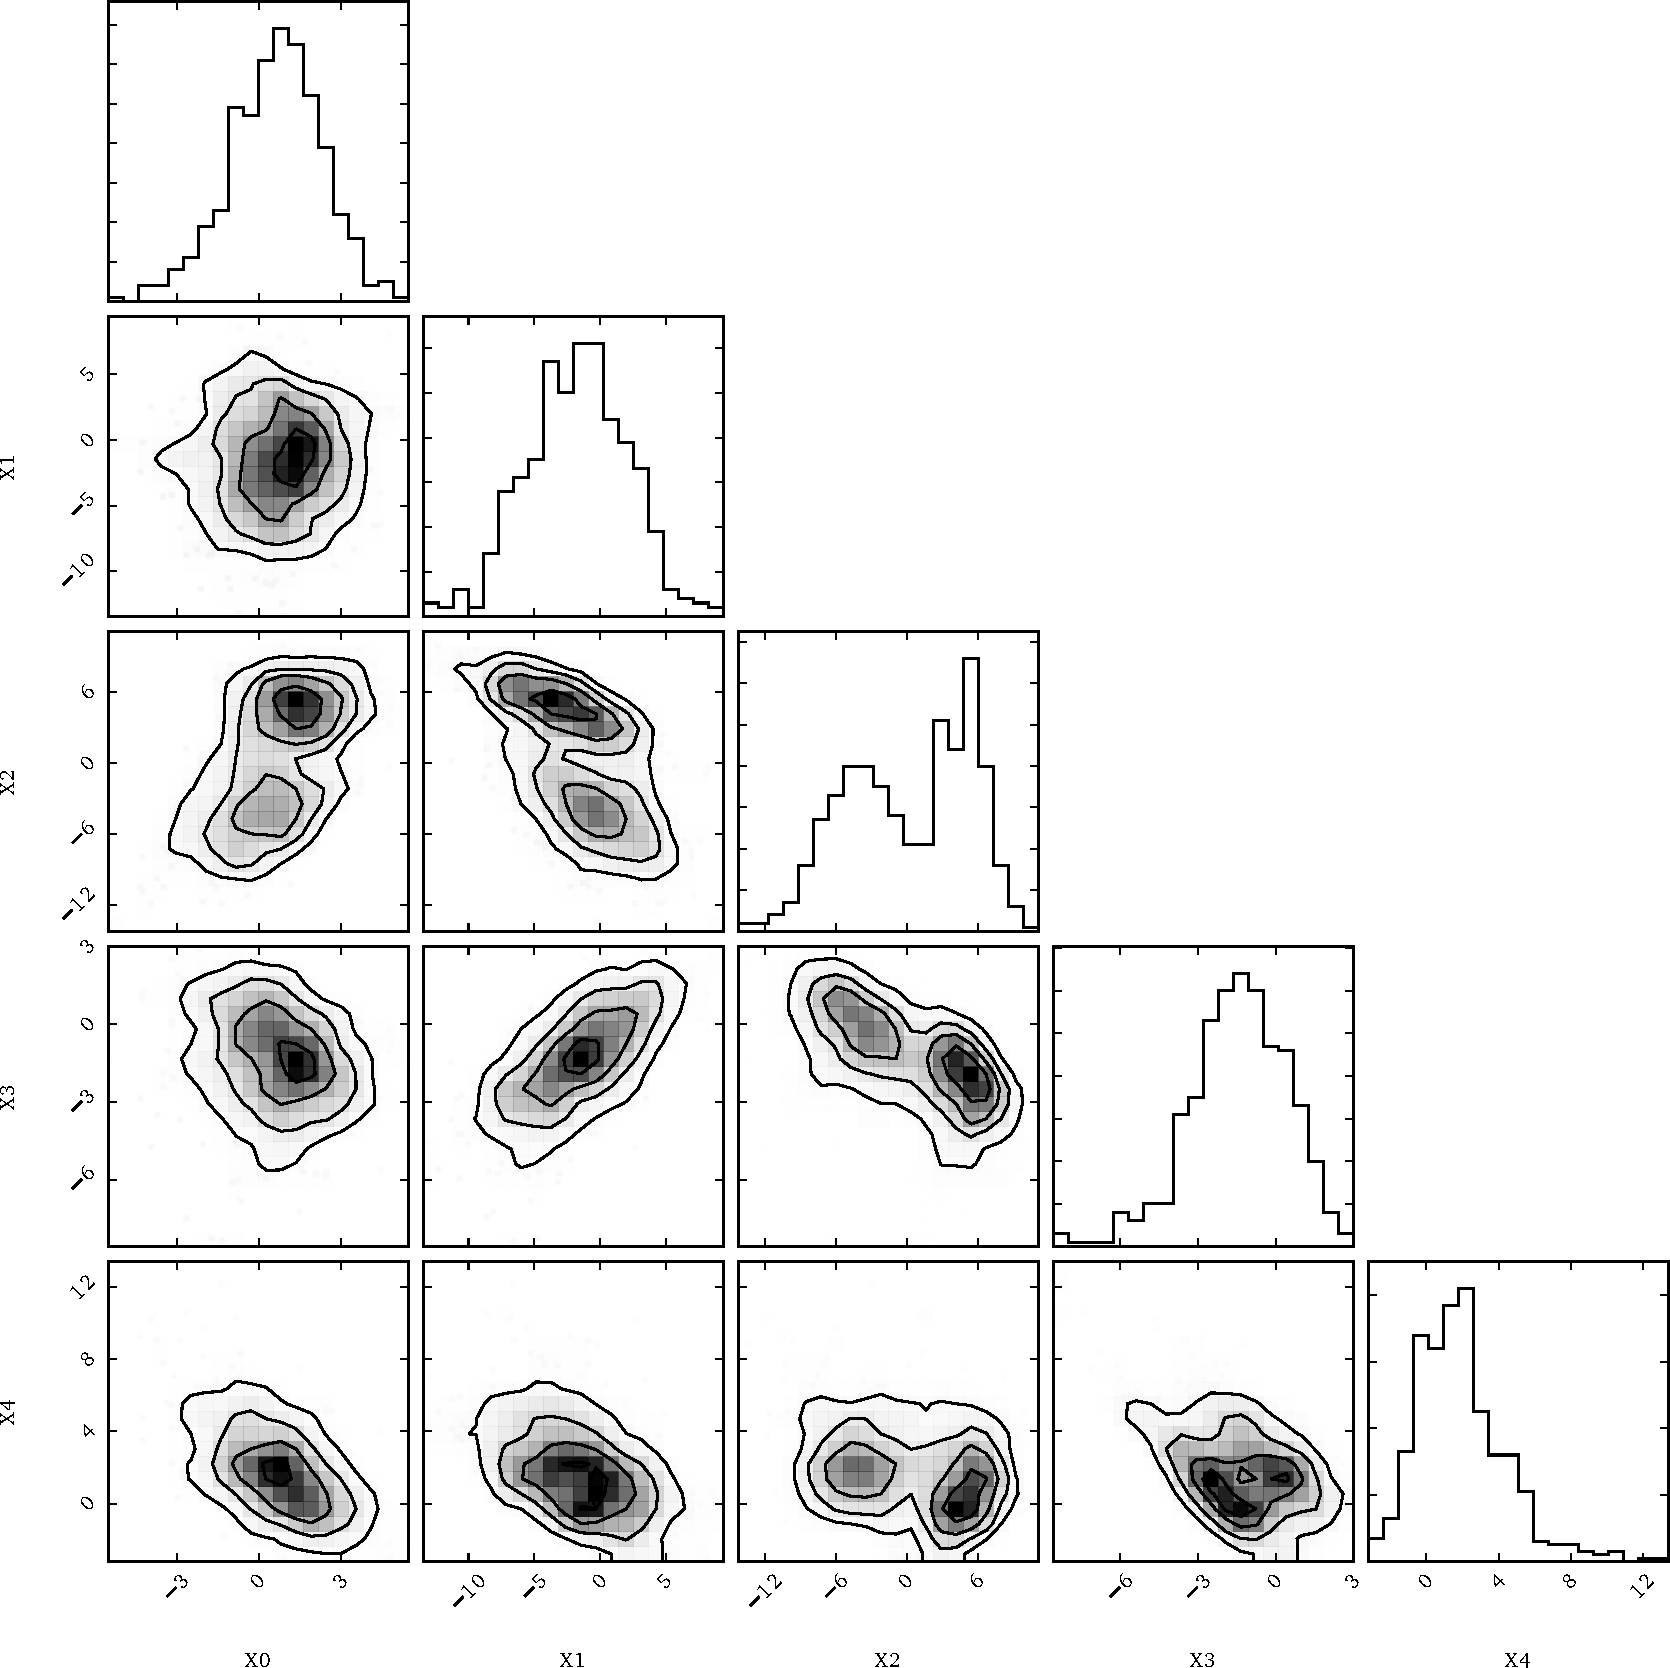
\includegraphics[width=\textwidth]{figures/fig4.pdf}\\
        Observed data ${\cal D}$
    \end{column}
\end{columns}

\end{frame}

\begin{frame}
    \frametitle{Example: Inference from multidimensional data}

    Recipe:

    \begin{enumerate}
        \item Build a single parameterized classifier $s(\mathbf{x}; \theta_0, \theta_1)$,
        in this case a 2-layer NN trained on 5+2 features, with the alternative fixed to $\theta_1=(\alpha=0, \beta=0)$.

        \item Find the approximated MLE $\hat \alpha, \hat \beta$ by solving Eqn.~\ref{eqn:mle}.
            \begin{itemize}
                \item Solve Eqn.~\ref{eqn:mle} using likelihood scans or through optimization.
                \item Since the generator is inexpensive, $p(s(\mathbf{x}; \theta_0, \theta_1)|\theta)$ can be calibrated on-the-fly, for every candidate $(\alpha,\beta)$, e.g. using histograms.
            \end{itemize}

        \item Construct the log-likelihood ratio (LLR) statistic
        \begin{equation*}
            -2 \log \Lambda(\alpha, \beta ) = -2 \log \frac{p({\cal D} | \alpha, \beta)}{  p({\cal D} | \hat \alpha, \hat \beta) }
        \end{equation*}

    \end{enumerate}

\end{frame}

\begin{frame}


    \begin{columns}
      \begin{column}[t]{0.48\textwidth}
        \centering
        \small Exact $-2 \log \Lambda(\alpha, \beta )$\\
        \vspace{0.5em}
        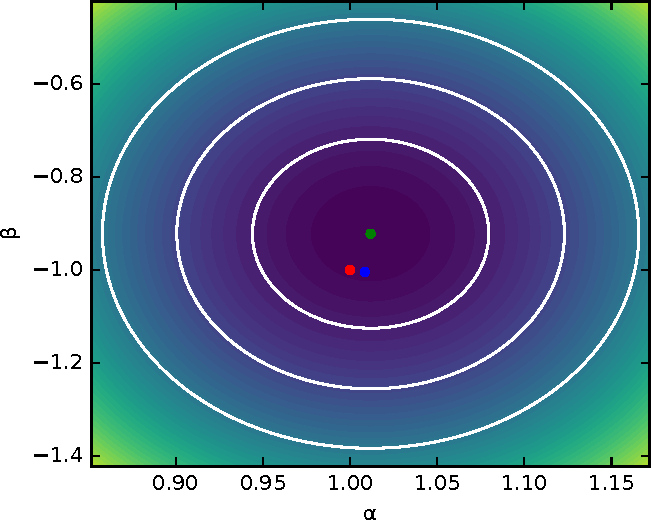
\includegraphics[height=10em]{figures/fig5a.pdf}
      \end{column}
      \begin{column}[t]{0.48\textwidth}
          \centering
          \small GP surrogate of the approx. LLR\\
          \vspace{0.5em}
          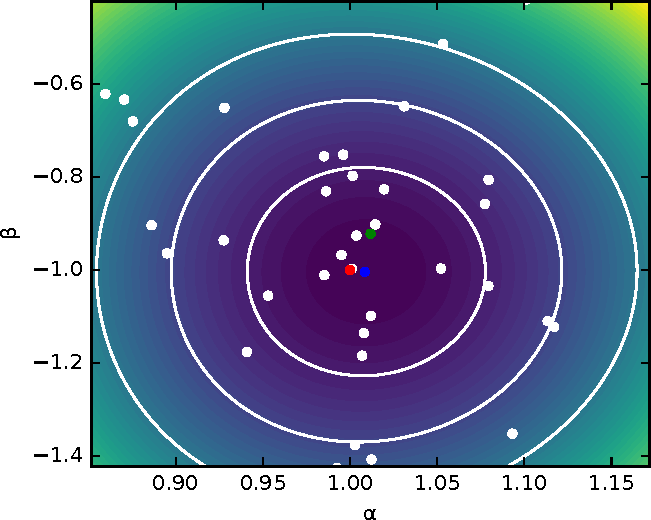
\includegraphics[height=10em]{figures/fig5c.pdf}
      \end{column}
    \end{columns}

    \vspace{1em}

    \centering
    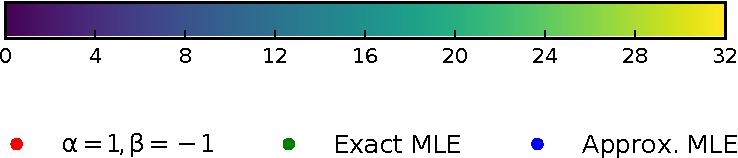
\includegraphics[width=0.5\textwidth]{figures/fig5d.pdf}

\end{frame}


\begin{frame}
    \frametitle{Summary}

    \begin{itemize}
        \item We proposed an approach for approximating LR in the likelihood-free setup.

        \item Evaluating likelihood ratios reduces to supervised learning. Both problems are deeply connected.

        \item Alternative to Approximate Bayesian Computation, without the need to define a prior over parameters.
    \end{itemize}
\end{frame}

\begin{frame}[plain,noframenumbering]
    \frametitle{References}
    {\footnotesize
    \bibliographystyle{apalike}
    \bibliography{biblio}}
\end{frame}





\end{document}
